% --- Conteúdo ATUALIZADO para Tabela&Grafico/shell_sort.tex ---

\qquad A seguir são apresentados os resultados obtidos na execução do algoritmo \textit{Shell Sort}.

% --- IMAGEM DA TABELA DO SHELL SORT ---
\begin{figure}[h!]
    \centering
    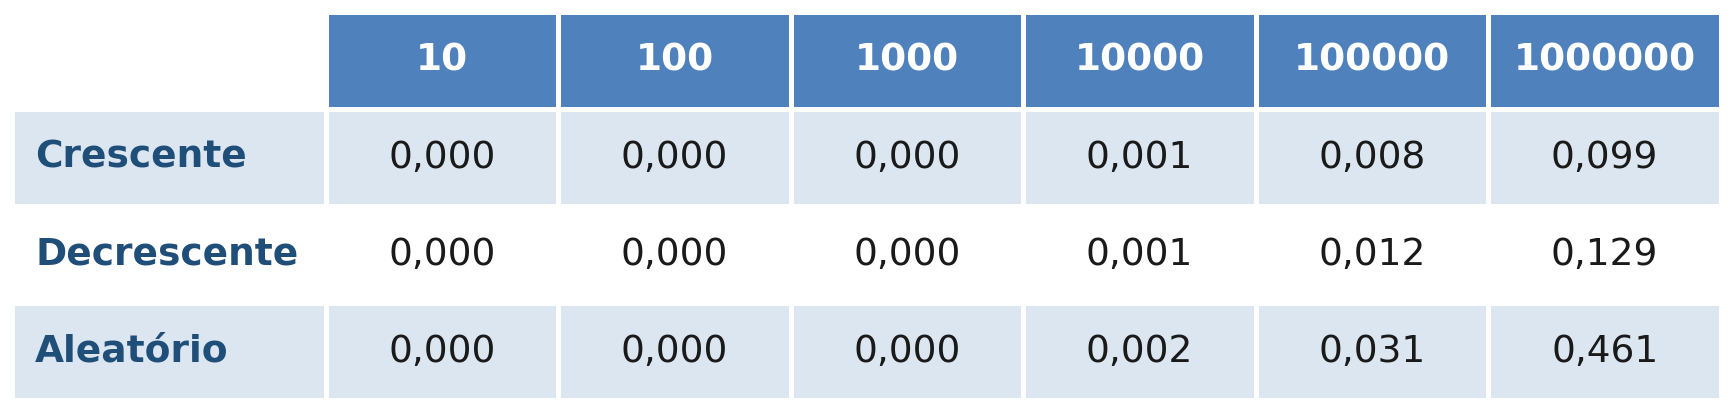
\includegraphics[width=1.0\textwidth]{Imagens/Shell_sort/tabela_shell.png}
    \caption{Tabela de tempo de execução (em segundos) do \textit{Shell Sort} (elaborado pelo autor).}
    \label{fig:tabela_shell}
\end{figure}

% --- IMAGEM DO GRÁFICO DO SHELL SORT ---
\begin{figure}[h!]
    \centering
    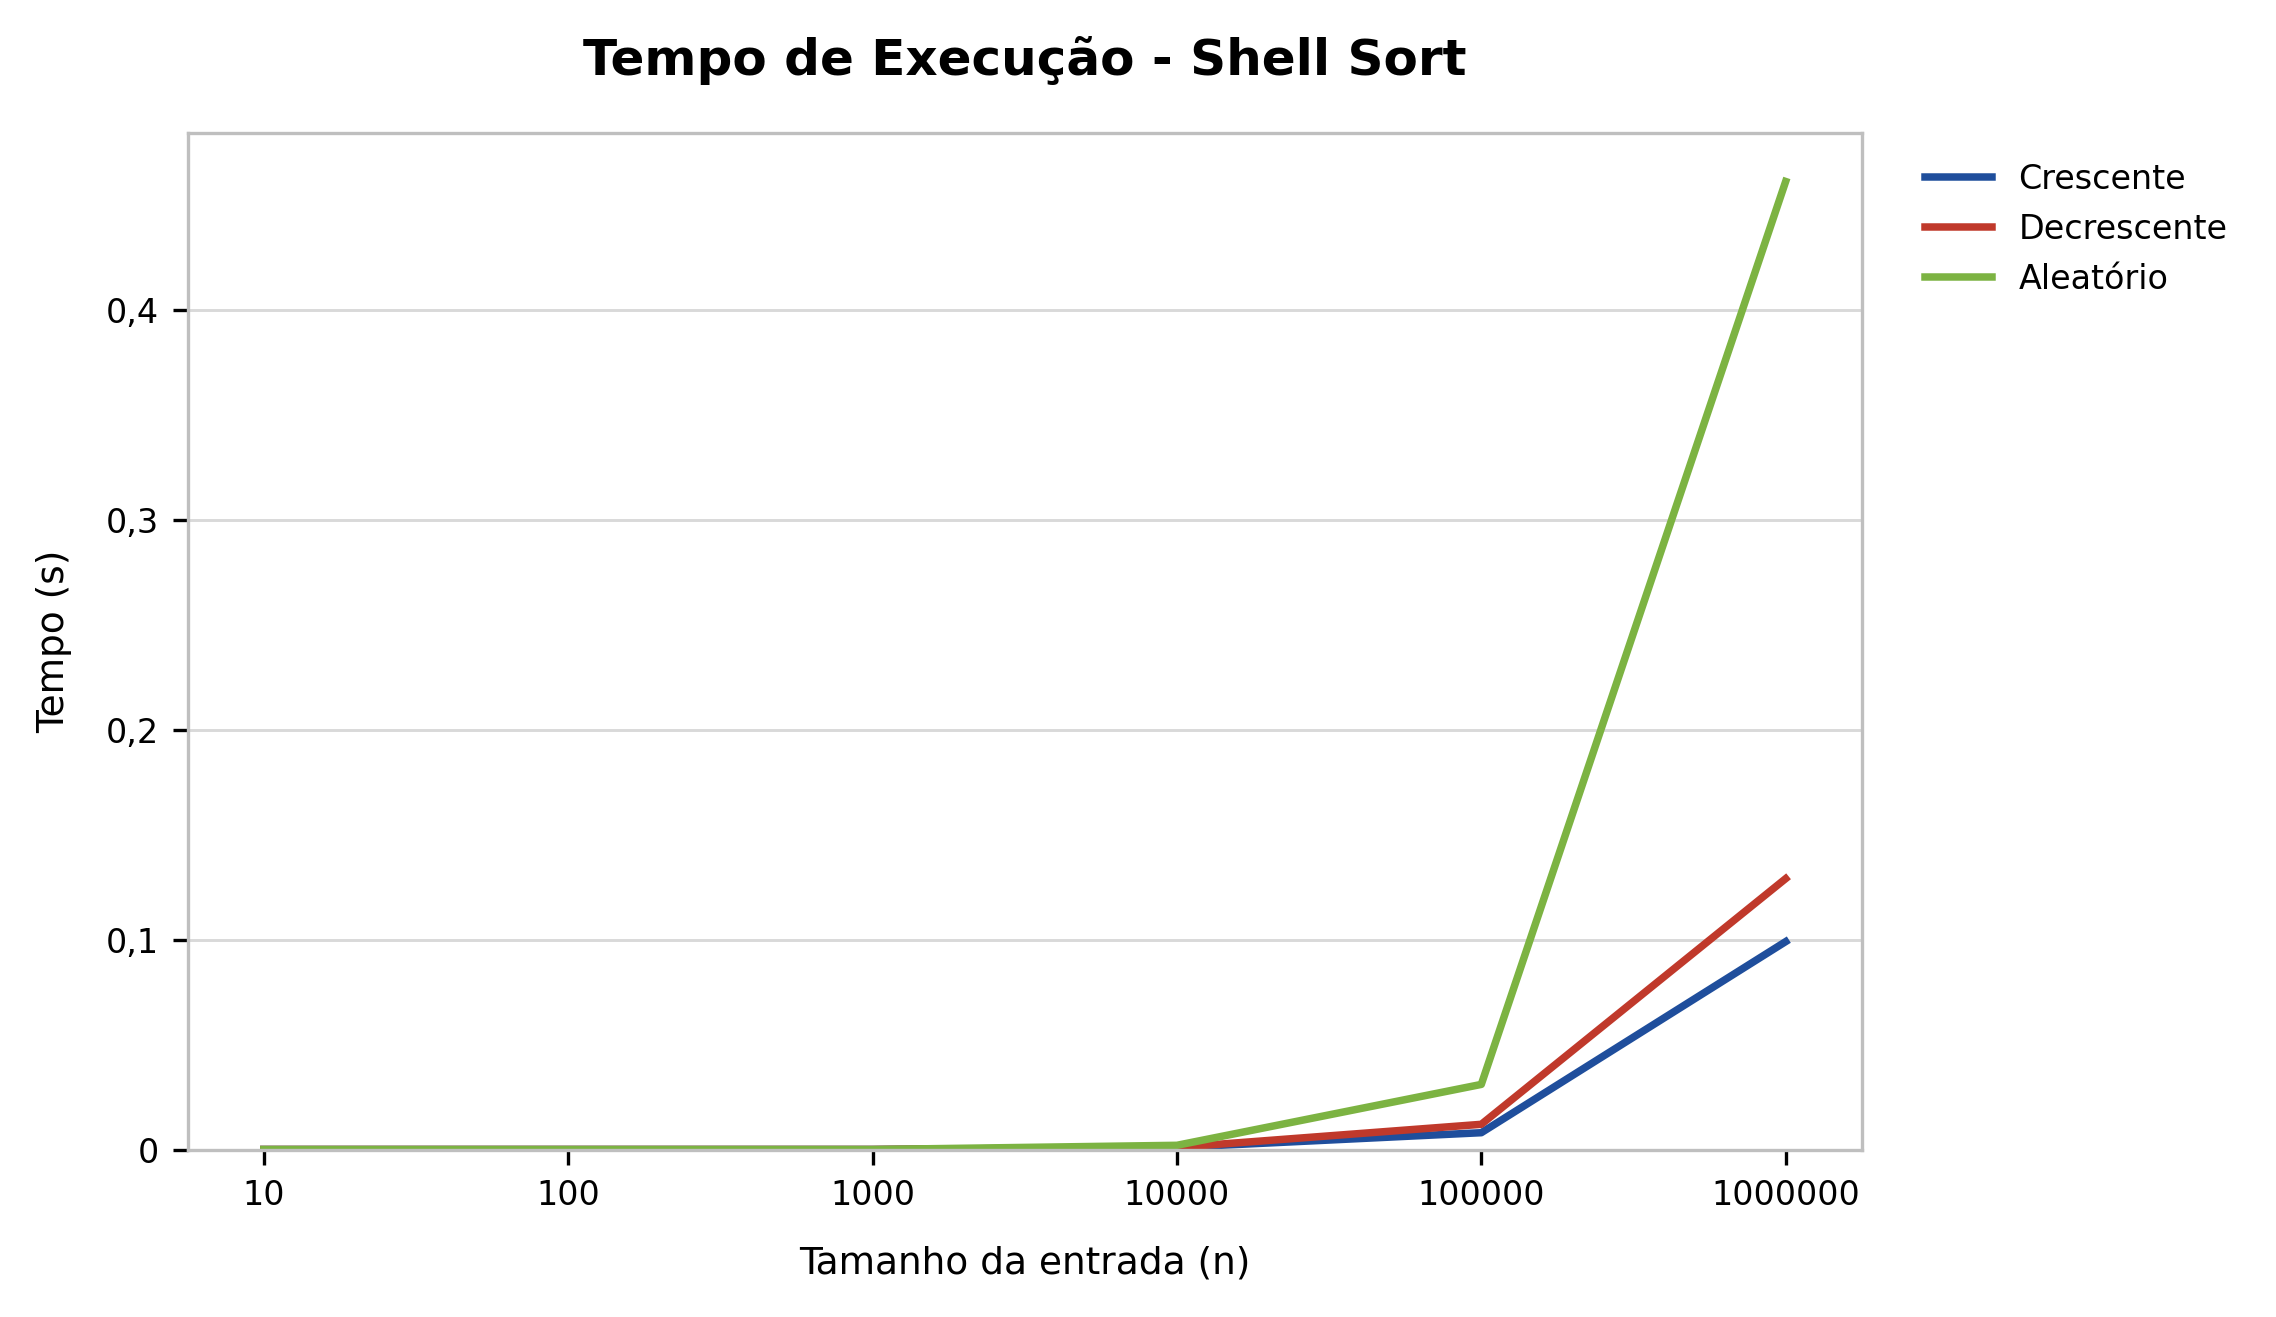
\includegraphics[width=1.0\textwidth]{Imagens/Shell_sort/grafico_shell.png}
    \caption{Desempenho do Algoritmo \textit{Shell Sort} (elaborado pelo autor).}
    \label{fig:grafico_shell}
\end{figure}

% --- ANÁLISE DOS RESULTADOS DO SHELL SORT ---

\qquad Os dados da Figura \ref{fig:tabela_shell} e o gráfico da Figura \ref{fig:grafico_shell} mostram uma diferença expressiva de desempenho em relação aos algoritmos quadráticos analisados anteriormente. Para as entradas de 10, 100 e 1.000 elementos, os tempos registrados foram de 0,000 segundo em todos os cenários, o que indica apenas que a duração ficou abaixo da precisão do relógio utilizado. Diferenças só passam a ser perceptíveis a partir de 10.000 elementos.

\begin{itemize}
    \item \textbf{Desempenho subquadrático:} para ordenar um milhão de elementos no cenário aleatório, o \textit{Shell Sort} levou 0,461 segundo, enquanto o \textit{Selection Sort} levou 1.658,270 segundos e o \textit{Bubble Sort}, 3.954,730 segundos. Isso representa um desempenho cerca de 3.600 e 8.600 vezes superior, respectivamente.

    \item \textbf{Crescimento dos tempos:} ao passar de 100.000 para 1.000.000 de elementos, entrada dez vezes maior, o tempo do caso aleatório passou de 0,031 s para 0,461 s, um crescimento de aproximadamente 15 vezes. Em um algoritmo quadrático, o mesmo aumento resultaria em um tempo cerca de 100 vezes maior, como de fato ocorreu com o \textit{Selection Sort}. Esse resultado é compatível com a complexidade esperada para a sequência de \textit{gaps} utilizada.

    \item \textbf{Influência da ordem inicial:} a ordem dos dados ainda afeta o desempenho, mas de forma muito menos acentuada. O vetor crescente foi o mais rápido (0,099 s), seguido pelo decrescente (0,129 s) e pelo aleatório (0,461 s). O cenário aleatório é o mais custoso porque os elementos precisam percorrer distâncias maiores até suas posições finais, enquanto nas entradas ordenada e invertida a estrutura regular dos dados permite deslocamentos mais previsíveis.
\end{itemize}

\qquad Os resultados mostram que o \textit{Shell Sort} é consideravelmente mais eficiente que os métodos quadráticos simples, mantendo tempos inferiores a um segundo mesmo para um milhão de elementos, o que o torna uma alternativa viável para conjuntos de dados de tamanho médio a grande.

\FloatBarrier